\documentclass[t,table,usenames,dvipsnames]{beamer}

\usetheme{CambridgeUS}
\usecolortheme{beaver}
\setbeamertemplate{navigation symbols}{}

\usepackage[utf8]{inputenc}
\usepackage[croatian]{babel}

\usepackage{datetime}
\renewcommand{\dateseparator}{.}
\newcommand{\todayiso}{\twodigit\day \dateseparator \twodigit\month \dateseparator \the \year}
\date{\todayiso}

\usepackage{listings}
\usepackage{graphicx}
\usepackage{subcaption}
\usepackage{multirow}
\usepackage{color}
\definecolor{LightGray}{gray}{0.9}
\captionsetup{compatibility=false}

\title[NKOSL]{Napredno korištenje operacijskog sustava Linux}
\author[Dominik Barbarić, Josip Domšić]{Dominik Barbarić, Josip Domšić\\{\small Nositelj: doc.dr.sc. Stjepan Groš}}
\subtitle{3. Protokoli}
\institute[FER]{Sveučilište u Zagrebu\\Fakultet elektrotehnike i računarstva}

\begin{document}
{
    \setbeamertemplate{footline}{}
	\begin{frame}
		\maketitle
	\end{frame}
}

\begin{frame}
    \frametitle{OSI RM}
	\framesubtitle{\texttt{Open Systems Interconnection Reference Model}}
    \begin{itemize}
        \item Fizički sloj - Ethernet, USB, ISDN, 802.11, Bluetooth
        \item Podatkovni sloj - Ethernet, PPP, CSMA/CA 
        \item Mrežni sloj - ICMP, IPsec, IPv4, IPv6, AppleTalk
        \item Transportni sloj - UDP, TCP
        \item Sjednički sloj - HTTP, SMTP, SIP, Telnet
        \item Prezentacijski sloj - MIME
        \item Aplikacijski sloj - NFS
    \end{itemize}

\end{frame}

\begin{frame}
    \frametitle{TCP/IP}
	\framesubtitle{\texttt{Transmission Contral Protocol over Internet Protocol}}
    Najrasprostranjenija implementacija
    \begin{itemize}
        \item Podatkovni sloj (Fizički i Podatkovni)
        \item Mrežni sloj
        \item Transportni sloj
        \item Aplikacijski sloj (Sjednički, Prezentacijski, Aplikacijski)
    \end{itemize}
\end{frame}


\begin{frame}
    \frametitle{TCP/IP}
    \includegraphics[width=0.75\textwidth]{tftp.jpg}
\end{frame}


\begin{frame}
	\frametitle{Komunikacija}
    \begin{itemize}
        \item IP protokol sadrži podatke o adresi, veličini paketa, \ldots
        \item TCP održava vezu između 2 subjekta / računala / hosta
        \item Jedinstveno definirano s: parom IP adresa i port
        \item Alternativa je socket file
        \item Definira se i tip komunikacije: Stream, Datagram, RAW, ...
    \end{itemize}
\end{frame}


\begin{frame}
    \frametitle{Klijent-Server arhitektura}
	\begin{itemize}
		\item Server pruža usluge klijentima preko definiranih mrežnih protokola
        \item Alternativa je peer-to-peer
		\begin{itemize}
			\item Serveru se pristupa preko \textit{socket}a
			\item[] IP adresa i port
			\item[] Prijenosni protokol (TCP, UDP, \ldots)
		\end{itemize}
		\item Serverski programi se pokreću kao \emph{daemon}
	\end{itemize}
\end{frame}


\begin{frame}
    \frametitle{Protokoli}
    \begin{itemize}
        \item INETD / XINETD 
        \item SSH
        \item HTTP
        \item FTP
        \item NFS, SMB
        \item DNS
    \end{itemize}
\end{frame}


\begin{frame}
	\frametitle{ssh}

	TCP port 22\\
	OpenSSH, Dropbear, \ldots

	\begin{itemize}
		\item Pristup udaljenoj sesiji
		\item Enkriptirani protokol
		
		\item SFTP i SCP protokoli
		\item SSH tunnel
		\item[] X11 forwarding
	\end{itemize}
\end{frame}

\begin{frame}[fragile]
	\frametitle{ssh}
	\framesubtitle{\texttt{/etc/ssh/sshd\_config}}
	\scriptsize
	\begin{verbatim}
Port 22
AddressFamily any
ListenAddress 0.0.0.0                      # IP adrese na kojima server slusa
ListenAddress ::                           #      IPv6

Protocol 2                                 # SSH-2 protokol

HostKey for protocol version 1
HostKey /etc/ssh/ssh_host_key              # Sigurnosni kljucevi servera
HostKeys for protocol version 2            # Koriste se za enkripciju veze
HostKey /etc/ssh/ssh_host_rsa_key
HostKey /etc/ssh/ssh_host_dsa_key
HostKey /etc/ssh/ssh_host_ecdsa_key
HostKey /etc/ssh/ssh_host_ed25519_key

SyslogFacility AUTH                        # Postavke logova
LogLevel INFO                              # Razina logiranja

PidFile /run/sshd.pid                      # Datoteka s PID-om servera
	\end{verbatim}


\end{frame}

\begin{frame}[fragile]
	\frametitle{ssh}
	\framesubtitle{\texttt{/etc/ssh/sshd\_config}}
	\scriptsize
	\begin{verbatim}
LoginGraceTime 600                          # Vrijeme cekanja prije ponovnog logina
PermitRootLogin no                         # Ogranicenja autentifikacije
StrictModes yes
axAuthTries 6
axSessions 10

# Odabir nacina autentifikacije korisnika
RSAAuthentication yes                      # RSA kljucevi
PubkeyAuthentication yes

# Datoteka s popisom kljuceva s dozvoljenim pristupom (za svakog korisnika)
AuthorizedKeysFile      .ssh/authorized_keys

RhostsRSAAuthentication no                 # Autentifikacija klijentskih racunala
HostbasedAuthentication no
	\end{verbatim}

\end{frame}

\begin{frame}[fragile]
	\frametitle{ssh}
	\framesubtitle{\texttt{/etc/ssh/sshd\_config}}
	\scriptsize
	\begin{verbatim}
# Onemogucavanje tekstualnih sifri
# Cesto "no" ako se koriste druge metode autentifikacije
PasswordAuthentication no
PermitEmptyPasswords no
ChallengeResponseAuthentication no

# Autentifikacija kroz druge auth protokole
KerberosAuthentication no
GSSAPIAuthentication no
UsePAM yes

# Omogucen X11 forward za X klijente na serveru
X11Forwarding yes

	\end{verbatim}

\end{frame}


\begin{frame}
	\frametitle{telnet}

	TCP port 23\\
	xinetd
	
	\begin{itemize}
		\item Udaljeni pristup konzoli
		\item Nesiguran protokol
		
		\item Često korišten na ugradbenoj opremi
	\end{itemize}
\end{frame}


\begin{frame}
	\frametitle{vnc}

	TCP port 5900\\
	tightvnc, tigervnc, realvnc

	\begin{itemize}
		\item Virtual Network Computing
		\item Udaljeni pristup grafičkom sučelju
		
		\item Koristi Remote Framebuffer protokol
		\begin{itemize}
			\item Rad s bilo kojim windowing sustavom
		\end{itemize}
	\end{itemize}
\end{frame}

\begin{frame}
	\frametitle{vnc}
	\centering
	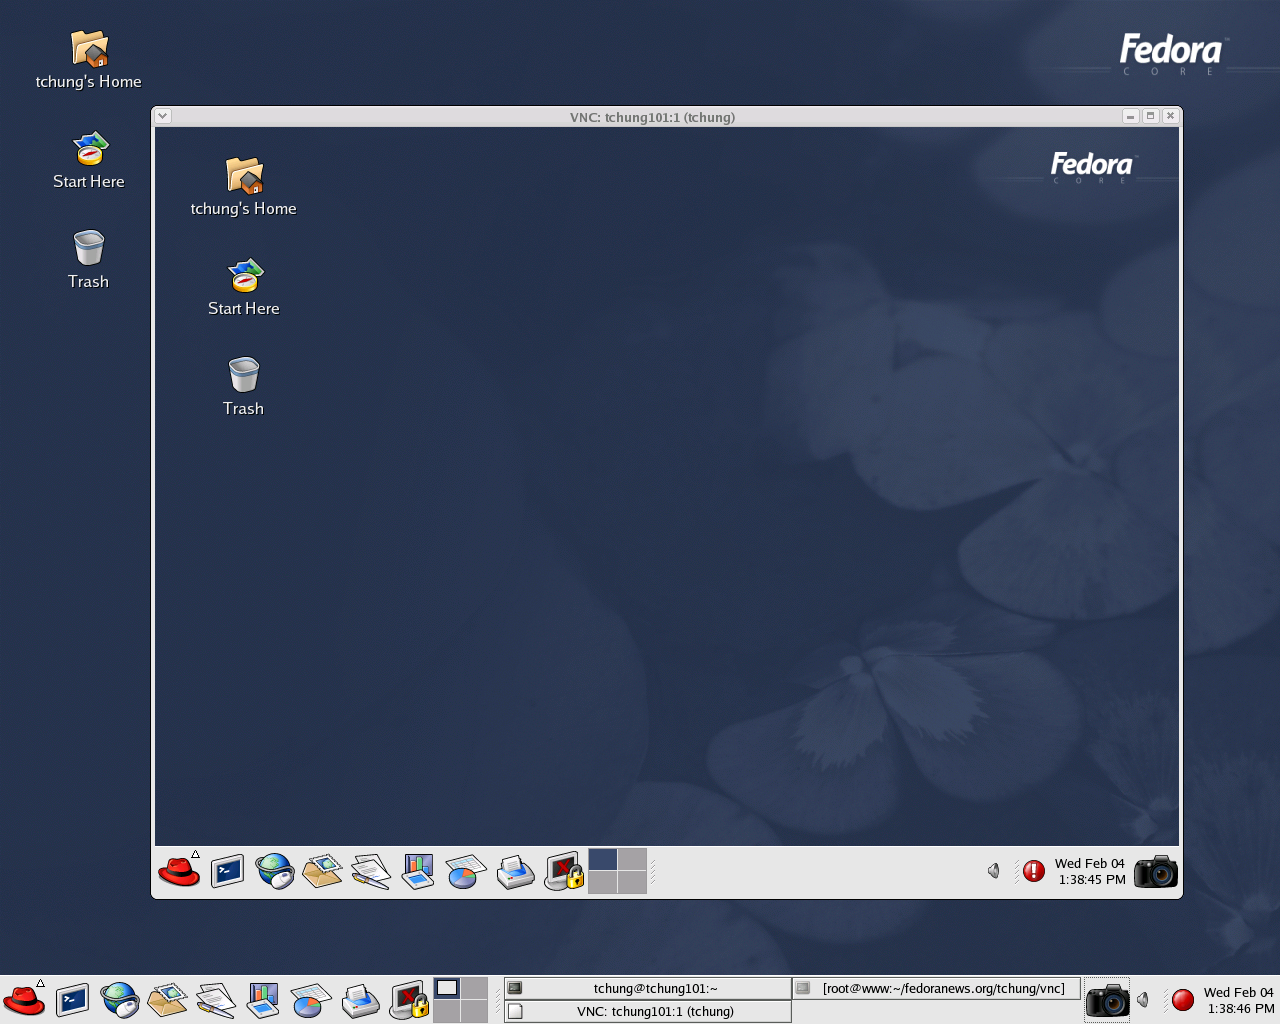
\includegraphics[width=0.75\textwidth]{vnc-desktop.png}

\end{frame}


\begin{frame}
	\frametitle{ftp}
	
	TCP port 21 (control)\\
	vsftpd, proftpd, bftpd, \ldots

	\begin{itemize}	
		\item File Transfer Protocol
		\item Varijante: TFTP, SFTP (SSH FTP), FTPS (SSL/TLS FTP)
		
		\item Dva načina rada:
		\begin{itemize}
			\item Aktivni
			\item Pasivni
		\end{itemize}
	\end{itemize}
\end{frame}

\begin{frame}
	\frametitle{ftp}
	\framesubtitle{Način rada}
	\centering
	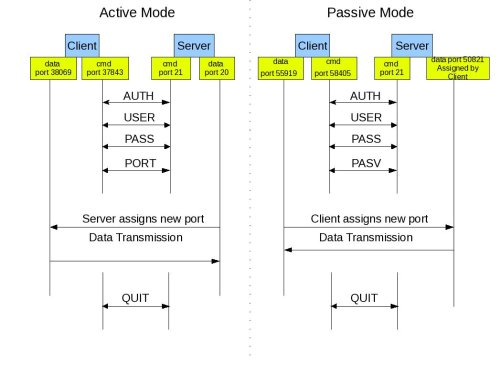
\includegraphics[width=0.85\textwidth]{ftp.jpg}
\end{frame}


\begin{frame}[fragile]
	\frametitle{ftp}
	\framesubtitle{\texttt{/etc/vsftpd.conf}}
	\scriptsize
	\begin{verbatim}
anonymous_enable=NO                       # Anonimni pristup
local_enable=YES                          # Pristup lokalnim korisnicima

# Per-user configuration
user_config_dir=/etc/vsftpd_conf.d        # Folder u kojem se nalaze konfiguracije
                                          # za svakog korisnika

# Omogucena FTP write naredba (dozvola pisanja na server)
write_enable=YES
# Don’t allow recursive listing – prevents excessive I/O usage.
ls_recurse_enable=NO

# Logiranje uploada i downloada u xfer formatu
xferlog_enable=YES
xferlog_std_format=NO
log_ftp_protocol=YES

# ftp data kroz port 20 (active mode)
connect_from_port_20=YES
	\end{verbatim}

\end{frame}


\begin{frame}[fragile]
	\frametitle{ftp}
	\framesubtitle{\texttt{/etc/vsftpd.conf}}
	\scriptsize
	\begin{verbatim}
# Uploaded files are owned by the uploader.
chown_uploads=NO

# You may change the default value for timing out an idle session.
idle_session_timeout=600

# You may change the default value for timing out a data connection.
data_connection_timeout=120

# Location of the RSA certificate to use for SSL encrypted connections.
rsa_cert_file=/etc/ssl/private/vsftpd.pem

# Allow PASV (passive ftp)
pasv_enable=YES
pasv_min_port=12000                      # Dozovljeni portovi u pasivnom modu
pasv_max_port=12500
pasv_address=123.45.678.901              # Javna adresa servera
pasv_addr_resolve=NO
# Allow active ftp
port_enable=YES
	\end{verbatim}


\end{frame}

\begin{frame}
	\frametitle{http}
	
	TCP port 80, 443\\
	Apache, Nginx
	
	\begin{itemize}
		\item[] HyperText Transfer Protocol
		
		\item[] Port 80 - neenkriptirana veza
		\item[] Port 443 - SSL veza
	\end{itemize}
	
	\begin{itemize}
		\item[] Apache konfiguracija \texttt{/etc/httpd/conf}
		\item[] Nginx konfiguracija \texttt{/etc/nginx}
	\end{itemize}

\end{frame}


\begin{frame}[fragile]
	\frametitle{Apache}
	\framesubtitle{\texttt{/etc/httpd/conf/httpd.conf}}
	\scriptsize
	\begin{verbatim}
Listen 80                                   # Port servera     

ServerRoot "/srv/apache"
DocumentRoot "/srv/apache/www"

ServerName localhost:80
ServerAdmin admin@example.com

ErrorLog logs/error.log                     # Postavke logiranja
LogLevel error

LoadModule cgi_module modules/mod_cgi.so
LoadModule dav_module modules/mod_dav.so
LoadModule dav_fs_module modules/mod_dav_fs.so
LoadModule dir_module modules/mod_dir.so
LoadModule mime_module modules/mod_mime.so

DefaultType text/plain                      # Defaultni MIME type
	\end{verbatim}

\end{frame}

\begin{frame}[fragile]
	\frametitle{Apache}
	\framesubtitle{\texttt{/etc/httpd/conf/httpd.conf}}
	\tiny
	\begin{verbatim}
<IfModule dir_module>
   DirectoryIndex index.html index.php index.aspx
</IfModule>

IndexIgnore .htaccess                                 # .htaccess datoteka nije index

<FilesMatch "^.ht">                                   # Zabrani pristup .htaccess datotekama
   Order allow,deny
   Deny from all
</FilesMatch>

<Directory />
   Options FollowSymLinks
   AllowOverride all
   Order deny,allow
   Allow from all
   Satisfy all
</Directory>

<Directory "/srv/apache/www/phpMyAdmin">              # Razlicite postavke za direktorij
   Options None
   AllowOverride None
   order deny,allow
   deny from all
   allow from 127.0.0.1
</Directory>
	\end{verbatim}

\end{frame}



\begin{frame}[fragile]

\frametitle{DHCP, DNS}

DHCP serveri
\begin{itemize}
	\item dhcpd, dnsmasq
\end{itemize}

DNS serveri
\begin{itemize}
	\item BIND, pdnsd, dnsmasq
\end{itemize}

\vfill

Primjer konfiguracije \texttt{/etc/dhcpd.conf}	
	\tiny
	\begin{verbatim}
# Postavke za sve rangeove koje router dodjeljuje
option domain-name-servers 8.8.8.8, 8.8.4.4;             # Adresa DNS-a koja se predaje klijentima
option subnet-mask 255.255.255.0;
option routers 139.96.30.100;                            # Gateway

# Postavke IP rangea
subnet 139.96.30.0 netmask 255.255.255.0 {
    range 139.96.30.150 139.96.30.250;
	
    host racunalo1 {                                     # Fiksna IP adresa za određenu MAC adresu
        hardware ethernet 70:56:81:22:33:44;
        fixed-address 139.96.30.199;
    }
}
	\end{verbatim}

\end{frame}



\begin{frame}
	\frametitle{Literatura}
	\url{https://wiki.archlinux.org/index.php/Server}
	\vfill
	\url{https://wiki.archlinux.org/index.php/vsftpd}\\
	\url{https://www.centos.org/docs/5/html/Deployment_Guide-en-US/s1-ftp-vsftpd-conf.html}\\
	\vfill
	\url{http://www.tldp.org/LDP/solrhe/Securing-Optimizing-Linux-RH-Edition-v1.3/chap15sec122.html}\\
	\vfill
	\url{https://wiki.archlinux.org/index.php/tightvnc}\\
	\vfill
	\url{https://wiki.archlinux.org/index.php/Dhcpd}\\
	\url{http://www.linuxhomenetworking.com/wiki/index.php/Quick_HOWTO_:_Ch08_:_Configuring_the_DHCP_Server}
\end{frame}

\end{document}
